\chapter{Auswertung}\label{Chap:Eval}
Im Folgenden soll betrachtet werden, wie gut der beschriebene Detektor 
in der Lage ist, Situationen wie in Abschnitt~\ref{chap:background-sec:Prob}
beschrieben zu erkennen. Dabei werden sowohl künstlich konstruierte 
Situationen, als auch tatsächliche Programme betrachtet. Für die Betrachtung 
tatsächlicher Programme werden Programme aus Goker~\cite{gobench}
verwendet. Dieses besitzt eine Sammlung von Programmteilen mit 
Concurrency-Bugs aus 9 
großen open-source Anwendungen wie z.B. Kubernetes und Moby. 
Beschreibungen der Probleme, sowie die Ergebnisse des Detektors befinden in 
Anhang~\ref{Appendix-1}.

\section{Standardprogramme}
Für die Analyse wurden insgesammt 43 Standartprobleme betrachtet. 
Dabei wurde überprüft, ob der Detektor in der Lage ist, das in dem 
Programm erhaltene Problem richtig zu erkennen, bzw.~zu erkennen wenn 
die vorliegende Situation nicht zu einem Problem führen kann. Eine 
tabellarische Beschreibung der betrachteten Situationen, sowie der Ergebnisse 
des Detektors ist in Tab.~\ref{App-Stand-Res} in Anhang~\ref{Appendix-1} aufgeführt.\\\\
Von den 43 Programmen konnten 39 korrekt kategorisiert werden. Dabei 
bestehen 18 Probleme aus Problemen mit Mutexen,
18 aus Problemen mit Channel und 7 mit einem 
Mix aus Mutexen und Channel. Abbildungen~\ref{Chap:Eval-Sec:Stand-Fig:Total}
bis~\ref{Chap:Eval-Sec:Stand-Fig:Mix} geben an, welcher Anteil der 
Betrachteten Standartprobleme korrekt erkannt wurde.\\\\
Für Programme, bei denen der Fehler auf die Verwendung von Mutexen 
basiert, konnten 17 der 18 Probleme richtig kategorisiert werden. 
Dies entspricht ca. $94.4\%$.\\
Bei den Programmen, bei welchen es durch Channel zu Problemen kommen kann, 
konnten ebenfalls 17 der 18 Programme.\\
Bei Programmen, welche sowohl Mutexe als auch Channels verwenden liegt 
die Erfolgsquote mit 5 aus 7 ($71.4\%$) am niedrigstem. Da der Detektor 
zwei verschiedene Methoden verwendet, um Probleme mit Mutexen und Probleme 
mit Channels zu erkenne, aber keine direkte Methode für die Erkennung
von Problemen besitzt, welche durch eine Kombination der beiden entstehen, 
werden solche Situationen nicht direkt erkannt. Sie werden nur dann erkannt, 
wenn sie dazu führt, dass einer der beiden Mechanismen sie erkennen 
kann. Es ist daher nicht verwunderlich, dass hierbei eine höhere Fehlerquote 
betrachtet werden kann, als wenn man die beiden Situationen einzeln
betrachtet.\\
Insgesamt hat der Detektor für die betrachteten Programme eine 
Trefferwahrscheinlichkeit von $90.7\%$. \\
Es sei noch dazu gesagt, dass die betrachteten Programme immer so implementiert 
worden sind, dass die entsprechenden Situationen auch in dem Durchlauf 
auftreten. Es ist allerdings auch möglich, dass Situationen bei den Durchläufen 
nicht durchlaufen werden, z.B. wenn sie sich ein einem Konditionellen 
Block (If) befinden, bei welchem die Bedingung während keinem der Durchläufe 
wahr wird. Da die entsprechenden Operationen somit nicht aufgezeichnet 
werden können, ist es demnach logischerweise auch nicht möglich, dass der 
Detektor die entsprechenden Situationen erkennt.




\begin{minipage}{0.45\textwidth}
  \centering  
  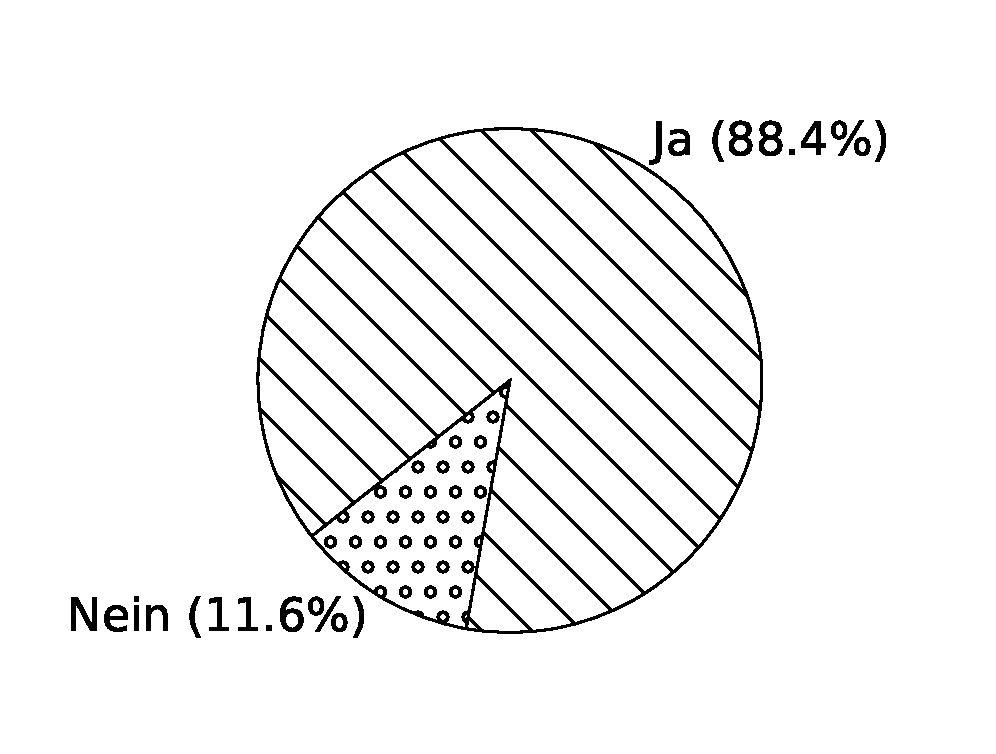
\includegraphics[width=0.8\textwidth]{img/pi_standard_total.eps}
  \captionof{figure}{Verteilung der Ergebnisse für Standardprogramme}
  \label{Chap:Eval-Sec:Stand-Fig:Total}
\end{minipage}
\hfill
\begin{minipage}{0.45\textwidth}
  \centering
  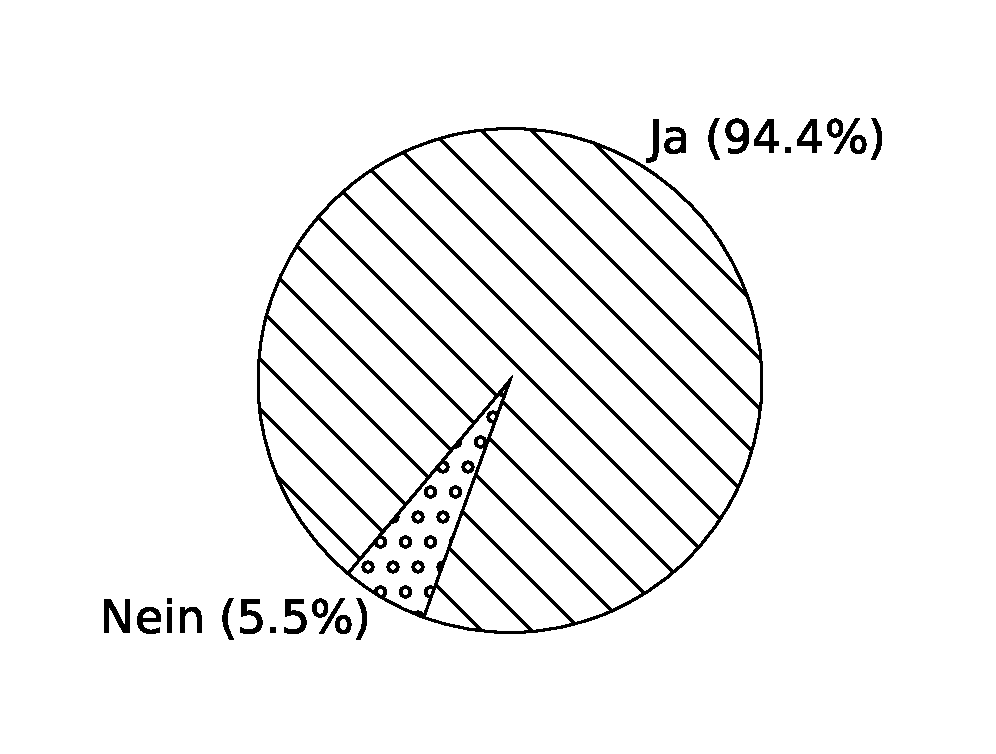
\includegraphics[width=0.8\textwidth]{img/pi_standard_mutex.eps}
  \captionof{figure}{Verteilung der Ergebnisse für Standardprogramme mit Mutexen}
  \label{Chap:Eval-Sec:Stand-Fig:Mutex}
\end{minipage}
\begin{minipage}{0.45\textwidth}
  \centering  
  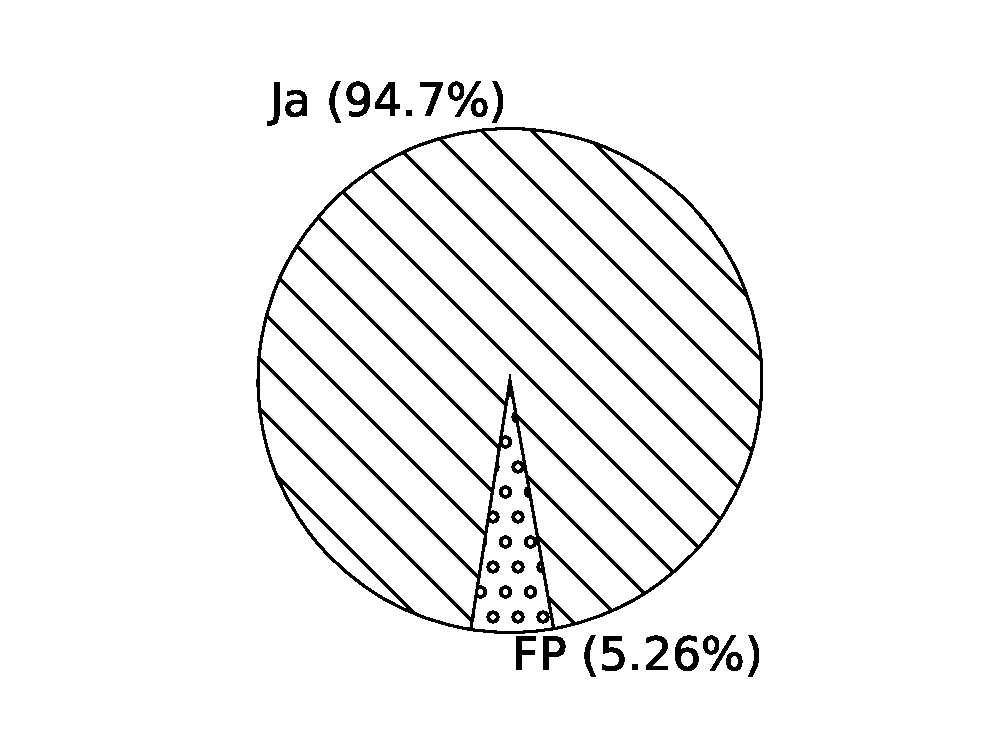
\includegraphics[width=0.8\textwidth]{img/pi_standard_channel.eps}
  \captionof{figure}{Verteilung der Ergebnisse für Standardprogramme mit Channel}
  \label{Chap:Eval-Sec:Stand-Fig:Channel}
\end{minipage}
\hfill
\begin{minipage}{0.45\textwidth}
  \centering
  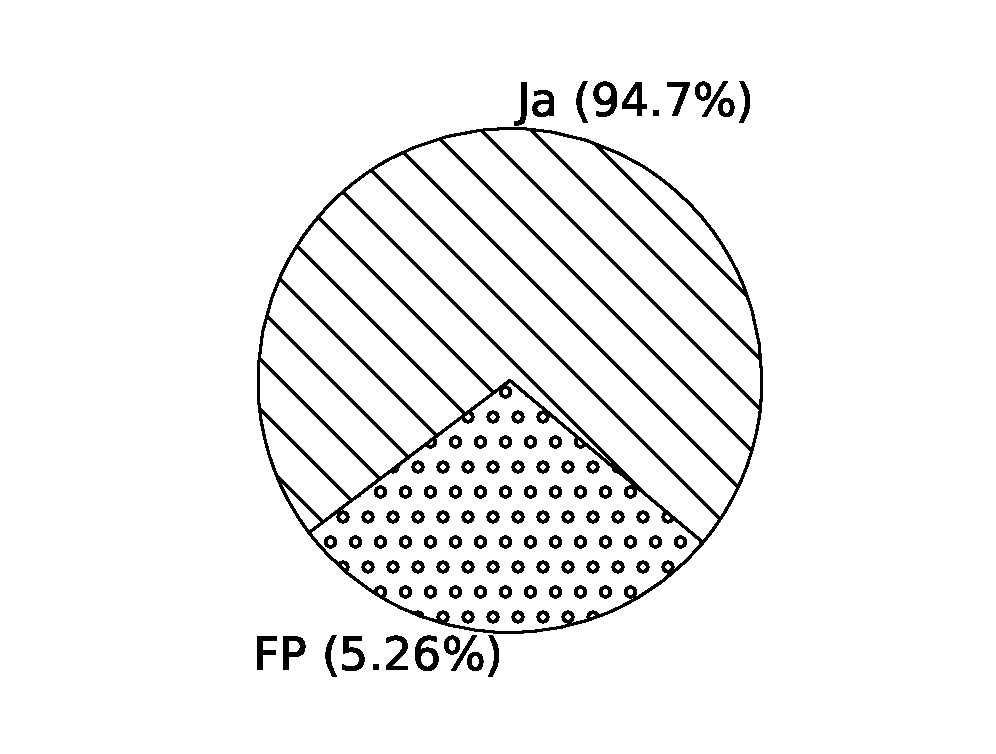
\includegraphics[width=0.8\textwidth]{img/pi_standard_mix.eps}
  \captionof{figure}{Verteilung der Ergebnisse für Standardprogramme mit Mutexen und Channel}
  \label{Chap:Eval-Sec:Stand-Fig:Mix}
\end{minipage}

\section{GoKer}
Für die Analyse wurden insgesamt 34 Programme betrachtet. Die betrachteten 
Programme und deren Ergebnisse befinden sich in Tab.~\ref{App-Goker} 
in Anhang~\ref{Appendix-1}. Von den Programmen betrafen 15 die 
Verwendung von Resource wie Mutexen (14 korrekt erkannt), 11 die 
Verwendung von Kommunikationen (10 korrekt erkannt) und 8 eine Kombination aus Mutexen und 
Channel (7 korrekt erkannt).
Die Erfolgsraten des Detektors für die Programme aus GoKer 
(Abb.~\ref{Chap:Eval-Sec:Goker-Fig:Total} bis~\ref{Chap:Eval-Sec:Goker-Fig:Mix})
stimmen dabei in etwa mit denen der Standardprogramme überein.
Für die Analyse wurden dabei nur solche Programme ausgewählt,
welche basieren auf ihrer Beschreibung für den Detektor theoretisch erkennbare 
Situation enthielt. Situationen, welche sich auf andere Concurrency-Bugs,
z.B. Race-Conditions bezogen wurden nicht betrachtet. 
Die Betrachtung der Programme aus Goker hat einen Nachteil der hier 
verwendeten Methode, bzw. der Implementierung deutlich gemacht.
Der Instrumenter ist nur in der Lage den vorliegenden Code zu instrumentieren. 
Es kann aber vorkommen, dass in einem Programm externe Funktionen 
verwendet werden, welche Mutexe oder Channel als Parameter oder 
Rückgabewerte besitzen. Da bei der Instrumentierung Mutexe und Channel 
durch eingens implementierte Objekte ersetzt werden, externe Funktionen 
aber nicht entsprechend Instrumentiert werden können kommt es 
hierbei zu Compiler-Fehlern. Die entsprechenden Programme sind daher nicht 
Lauffähig und können somit auch nicht analysiert werden. Programme aus GoKer, 
bei denen dies der Fall war wurden für die Analyse nicht betrachtet. 

\begin{minipage}{0.45\textwidth}
  \centering  
  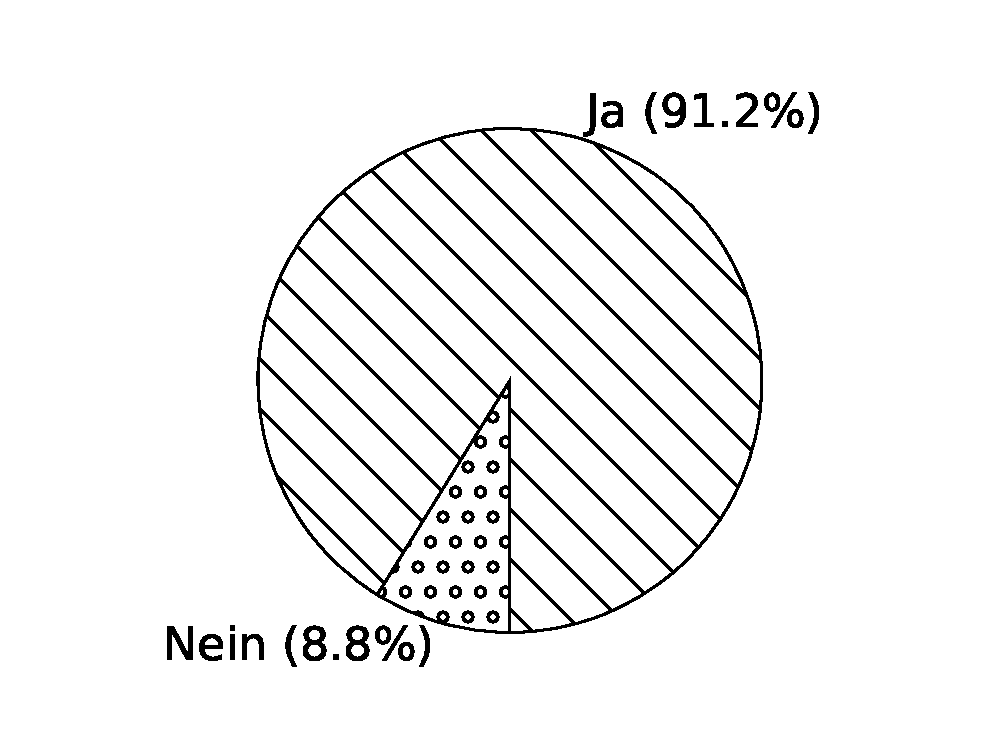
\includegraphics[width=0.8\textwidth]{img/pi_goker_total.eps}
  \captionof{figure}{Verteilung der Ergebnisse für Programme aus GoKer}
  \label{Chap:Eval-Sec:Goker-Fig:Total}
\end{minipage}
\hfill
\begin{minipage}{0.45\textwidth}
  \centering
  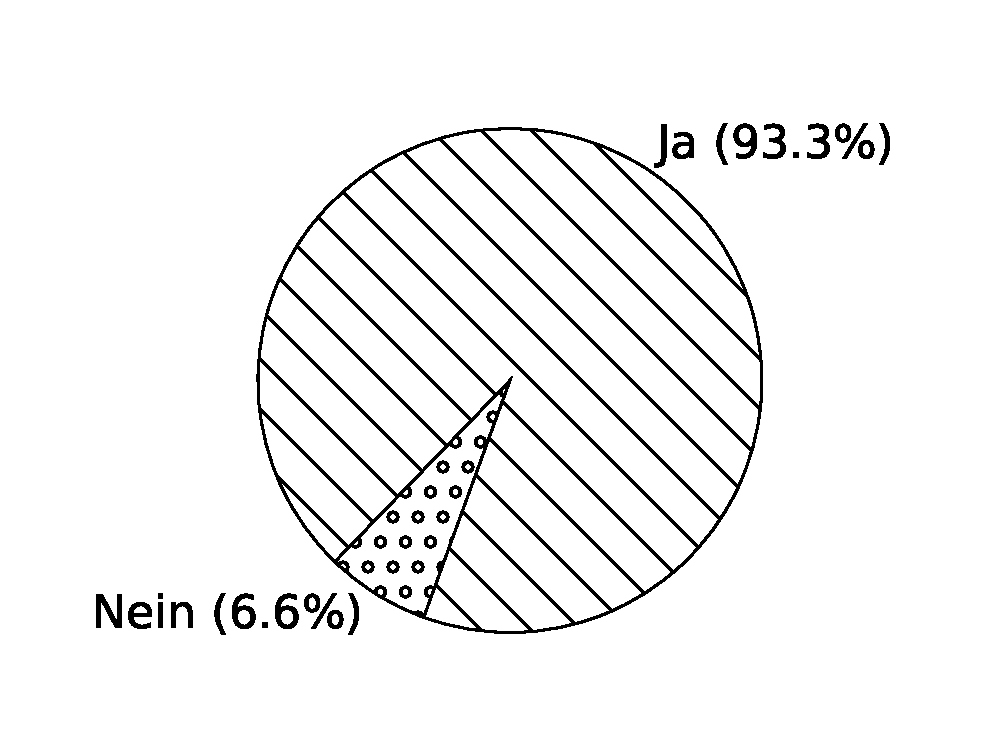
\includegraphics[width=0.8\textwidth]{img/pi_goker_mutex.eps}
  \captionof{figure}{Verteilung der Ergebnisse für Programme aus GoKer mit Mutexen}
  \label{Chap:Eval-Sec:Goker-Fig:Mutex}
\end{minipage}
\begin{minipage}{0.45\textwidth}
  \centering  
  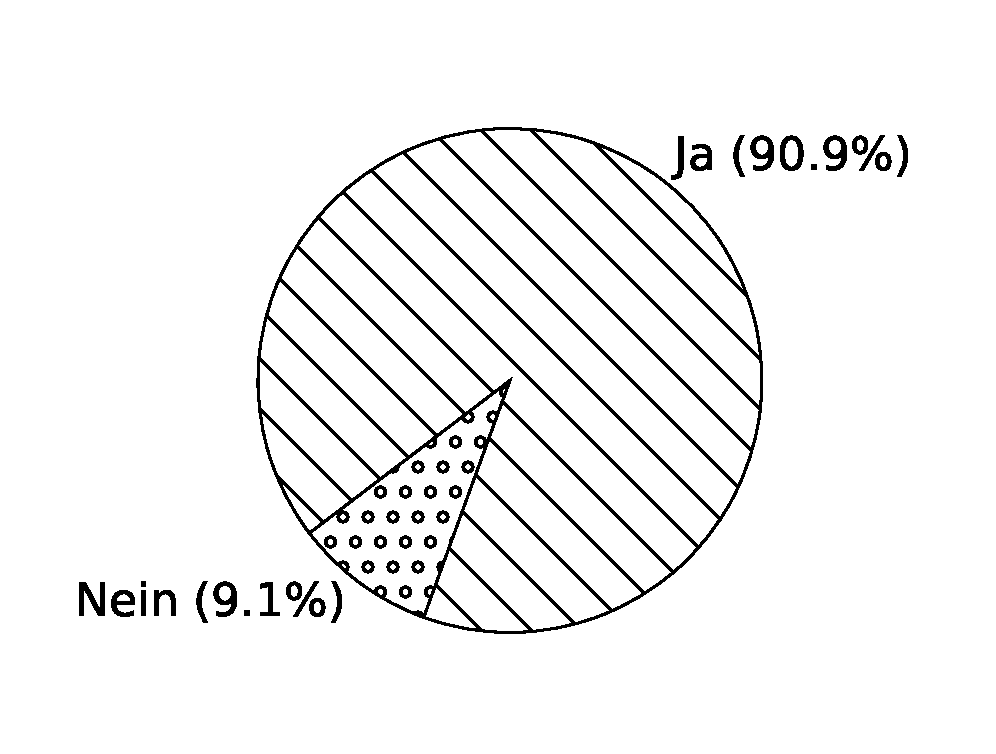
\includegraphics[width=0.8\textwidth]{img/pi_goker_channel.eps}
  \captionof{figure}{Verteilung der Ergebnisse für Programme aus GoKer mit Channel}
  \label{Chap:Eval-Sec:Goker-Fig:Channel}
\end{minipage}
\hfill
\begin{minipage}{0.45\textwidth}
  \centering
  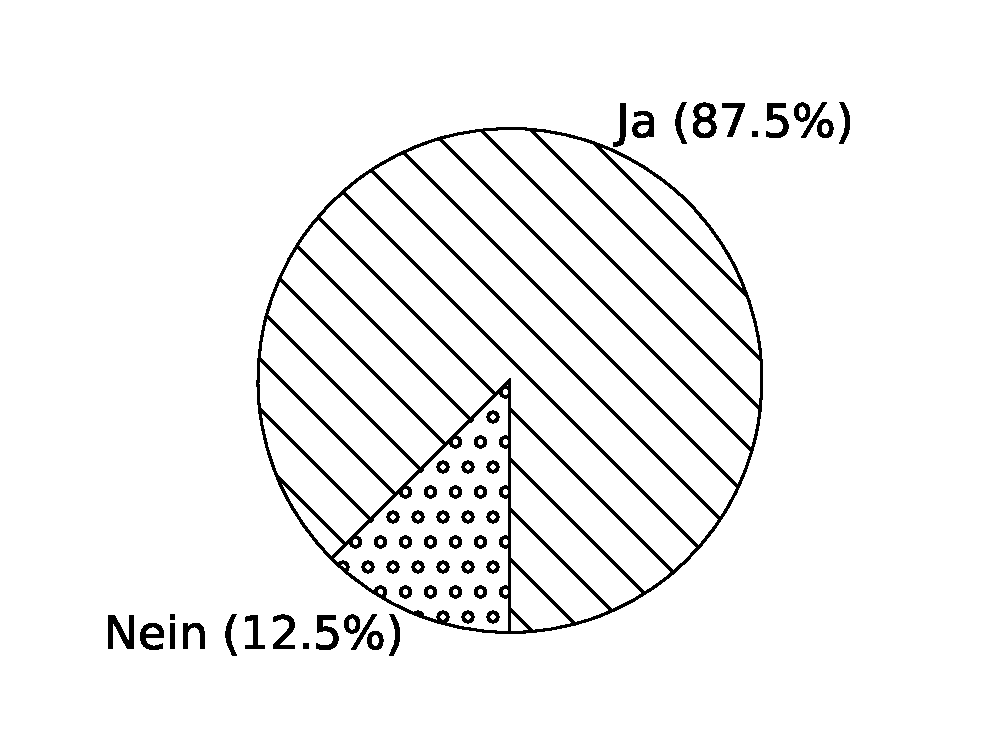
\includegraphics[width=0.8\textwidth]{img/pi_goker_mix.eps}
  \captionof{figure}{Verteilung der Ergebnisse für Programme aus GoKer mit Mutexen und Channel}
  \label{Chap:Eval-Sec:Goker-Fig:Mix}
\end{minipage}

\section{Probleme} \todo{Anderer Name}
\todo{Situationen, welche nicht betrachtet werden (z.B. in If, nach blockierender situation)}
\todo{Kommunikationene, welche in anderem Ablauf nicht möglich sind?}

Aufgrund der Funktionsweise des Implementers und der Analyse kann der Detektor 
momentan nur auf Probleme angewendet werden, welche durch 
\texttt{go build} kompiliert und anschließend direkt ausgeführt werden können.
Aus diesem Grund ist die direkte Anwendung des Detektors auf viele größere Programm 
in seinem momentanen Stand nicht möglich. 